\documentclass{report}

%%%%%%%%%%%%%     PACKAGES     %%%%%%%%%%%%%

\usepackage{marvin} %Custom Package by Marvin Lin
\usepackage{fancyhdr}

%%%%%%%%%%%%%     DOCUMNET FORMATTING     %%%%%%%%%%%%%

\pagestyle{fancy}
\fancyhf{}
\lhead{MTH261 Applied Linear Algebra}
\rhead{Marvin Lin}

%%%%%%%%%%%%%     TITLE, AUTHOR, ETC.     %%%%%%%%%%%%%

\title{MTH 261 Lecture Notes}
\author{Marvin Lin}
\date{Winter 2022}

%%%%%%%%%%%%%%%%%%%%%%%%%%%%%%%%%%%%%%%%%%%%%%%%%
%%%%%%%%%%%%%     DOCUMENT BODY     %%%%%%%%%%%%%
%%%%%%%%%%%%%%%%%%%%%%%%%%%%%%%%%%%%%%%%%%%%%%%%%

\begin{document}

\maketitle

\tableofcontents

\chapter{Introduction to Linear Algebra}
\section{System of Linear Equations}

Linear Algebra is the area of math concerning liner equations/functions that are represented in vector space and through matrices. If Calculus is the foundational language of mathematics, then Linear Algebra is the foundational language of STEM.

\begin{remark}
Keep in mind that while Linear Algebra utilizes matrices, it is just a tool to solve problems with. The study is \textbf{NOT} of matrices.
\end{remark}

\begin{definition}[Linear Equation]
An equation where $a_1x_1+a_2x_2+\dots+a_nx_n=b$, where $a_1,a_2,a_n, b \in$ as constants of $\mathbb{C}$ and in $\mathbb{R}$
\end{definition}

\begin{definition}[Linear System]
A collection of linear equations with the same variable
\end{definition}

\begin{definition}[Solution \& Solution Set]
A solution satisfies all equations in a system simultaneously, while a solution set is all possible solutions
\end{definition}

\begin{definition}[Equivalent Solutions]
Two systems with the same identical solution set
\end{definition}

\begin{definition}[Types of Solutions]
There are two major classification with solution, which are broken into three major solutions:
\begin{itemize}
	\item Inconsistent (no solutions)
	\item Consistent (at least one solution)
	\begin{itemize}
		\item Unique Solution
		\item Infinite Solutions
	\end{itemize}
\end{itemize}
Since the systems we are exploring and purely linear, there will not be two, three, or more solutions.
\end{definition}
\begin{figure}[h]

\begin{center}
  \includegraphics[width=10cm]{figures/solutions}
  \caption{Types of solutions in a linear system}
  \label{fig:graph1}
\end{center}
\end{figure}

\begin{remark}
This is true for all linear systems in all space
\end{remark}

\begin{definition}[Matrix]
A rectangular array of numbers, often used to compress systems. Let's say the following system of equations is given:
\begin{alignat*}{4}
 x & {}-{} & 7y & {} {} &    {}+{} & 6t & {}={} &  5 \\
   & {} {} &    & {} {} &  z {}-{} & 2t & {}={} & -3 \\
-x & {}+{} & 7y & {}-{} & 4z {}+{} & 2t & {}={} &  7
\end{alignat*}
It can be reduced into the following matrix:
\begin{equation*}
\begin{bmatrix}
1 & -7 & 0 & 6 \\ 
0 & 0 & 1 & -2 \\ 
-1 & 7 & -4 & 2
\end{bmatrix}
\end{equation*}
\end{definition}

\begin{definition}[Augmented Matrix]
A standard matrix which also includes the $\mathbf{b}$ coefficient in the matrix. The following is the augmented matrix of the system of equations from Definition 1.6:
\begin{equation*}
\begin{bmatrix}
1 & -7 & 0 & 6 \\ 
0 & 0 & 1 & -2 \\ 
-1 & 7 & -4 & 2
\end{bmatrix}
\;OR\;
\begin{bmatrix}
1 & -7 & 0 &\bigm| & 6 \\ 
0 & 0 & 1 &\bigm| & -2 \\ 
-1 & 7 & -4 &\bigm| & 2
\end{bmatrix}
\end{equation*}
\end{definition}

\section{Row Reduction and Echelon Forms}

\section{Vector Equations}

\section{The Matrix Equation $A\mathbf{x}=\mathbf{b}$}

\section{Solution Sets of Linear Systems}

\section{Linear Independence}

\section{Introduction to Linear Transformations}

\begin{definition}
A transformation $T$ is called linear (linear transformation) if for all $\mathbf{u}$, $\mathbf{v}$ in the domain of $T$ and c $\in \mathbb{R}$,
\begin{itemize}
	\item $T(\mathbf{u}+\mathbf{v}) = T(\mathbf{u} + T(\mathbf{v})$
	\item $T(c\mathbf{u}) = cT(\mathbf{u}$
\end{itemize}
Therefore, we can determine that every matrix transformation ($T(\mathbf{x} = A\mathbf{x})$ is a linear transformation
\end{definition}
To show that a transformation $T:\mathbb{R}^n \rightarrow \mathbb{R}^m$ is linear:
\begin{enumerate}
	\item Introduce $\mathbf{u}, \mathbf{v}\in\mathbb{R}^n and c\in\mathbb{R}.$ These must be arbitrary
	\item Show that $T(\mathbf{u}+\mathbf{v}) = T(\mathbf{u} + T(\mathbf{v}$
	\item Show that $T(c\mathbf{u}) = cT(\mathbf{u}$
\end{enumerate}
Turns out, we could show that IF WE ALREADY KNOW that $T$ is linear, then:
\begin{itemize}
	\item $T(\mathbf{0}) = \mathbf{0}$ and
	\item $T(c\mathbf{u}+d\mathbf{v}) = cT(\mathbf{u}) + dT(\mathbf{v}$
\end{itemize}
To show that $T$ is NOT linear, either:
\begin{itemize}
	\item Show $T(\mathbf{0}\neq\mathbf{0})$, or
	\item $T(\mathbf{u} + \mathbf{v}) \neq T(\mathbf{u}) + T(\mathbf{v})$ for specific vectors u \& v, or
\end{itemize}

\section{The Matrix of a Linear Transformation}

\begin{example}
Let $T:\mathbb{R}^2\rightarrow\mathbb{R}^2$ that first dilates vectors by a size of 2 then reflects across the line $x_2=-x_1$. Assuming this transformation is linear, find the standard matrix for $T$\\
\\
\textbf{Solution}
\begin{enumerate}
	\item Dilates (expands) by 2 $\rightarrow$ Doubles in size.
	\item Reflects across $x_1=-X_1 (y=-x)$.
\end{enumerate}
\end{example}

\chapter{Matrix Algebra}
\section{Matrix Operations}
There are several ways of representing a matrix:\\
\begin{center}
$\begin{bmatrix}
\mathbf{a}_1 & \mathbf{a}_2 & \dotsb & \mathbf{a}_n \\ 
\end{bmatrix}
=
\begin{bmatrix}
\mathbf{a}_ij
\end{bmatrix}
=
$
\end{center}
\begin{definition}
The \underline{diagonal entries} of the $m \times n$ matrix i
\end{definition}

\begin{definition}
The main diagonal is the collection diagonal entrias starting from the top left. \textbf{NOTE:} This may not include the bottom right due to the size of the matrix
\end{definition}

\begin{definition}
Diagonal matrix has the form:
\begin{equation*}
	\begin{bmatrix}
	\square & 0 & 0 & 0 \\ 
	0 & \square & 0 & 0 \\ 
	0 & 0 & \square & 0
	\end{bmatrix}
\end{equation*}
\end{definition}

\begin{definition}
The zero matrix is any matrix whos entries are all zero.
\end{definition}

Basic operations are the same between matrices and vectors (addition, subtraction, multiplication, and equality). Keep in mind, matrices must be the same size for addition/subtration operations.

\begin{example}[Properties of Matrix Arithmitic]
Let A, B, C, be matrices of the same size, $r,s,\in \mathbb{R}$.
\begin{enumerate}
	\item $A+B = B+A$
	\item $(A + B) + C = A + (B + C)$
	\item $A + O = A$
	\item $r(A +B) = rA +rB$
	\item $(r +s)A = rA +sA$
	\item $r(sA) = (rs)A$
\end{enumerate}
\textbf{NOTE:} $O$ is used a 0 in mathematics.
\end{example}

\subsection*{Matrix Multiplication}
When $B$ multiplies a vector $\mathbf{x}$ it starts from $\mathbf{x}\mapsto B\mathbf{x}$

\begin{definition}
If $A$ is $m \times n$ and $B$ is $n \times p$, then the product $AB$ is the $m \times p$ matrix.
\begin{center}
$AB = [A\mathbf{b}_1, A\mathbf{b}_2 \dots A\mathbf{b}_p]$
\end{center}
\end{definition}

\begin{remark}
The idea of non-communative multiplication is uncommon, however does occur on ocassion.
\end{remark}

\begin{example}
Let $A, B, C$ be matricies so that these are defined, $r \in \mathbb{R}$
\begin{enumerate}
	\item $A(BC) = (AB)C$
	\item $A(B + C) = AB + AC$
	\item $(B + C)A = BA + CA$
	\item $r(AB) = (rA)B = A(rB)$
	\item If $A$ is $m \times n$, then $I_mA = A = AI_n$
\end{enumerate}
\end{example}
\noindent A few common pitfalls. In general:
\begin{itemize}
	\item $AB \neq BA$
	\item Cancellation does not hold: $AB = AC \nRightarrow B = C$
	\item The Zero Product Principle does not hold: $AB = O \nRightarrow A = O$ or $B = O$
\end{itemize}
\begin{example}[Transpose Properties]
Let $A$, $B$, be matricies so that these are defined, $r \in \mathbb(R)$.
\begin{enumerate}
	\item $(A^T)^T = A$
	\item $(A + B)^T = A^T + B^T$
	\item $(rA)^T = rA^T$
	\item $(AB)^T = B^TA^T$
\end{enumerate}
\end{example}

\begin{remark}
This idea of ranposition will come up frequently in Linear Algebra.
\end{remark}

\section{The Inverse of a Matrix}
\begin{definition}[Multiplicative Inverse]
If $c \in \mathbb{R}$ with $c \neq O$,then:
\begin{center}
$c \cdot c^{-1} = 1$ and $c^{-1} \cdot c = 1$
\end{center}
In other words:
\begin{center}
	$A \cdot A^{-1} = I$ and $A^{-1} \cdot A = I$
\end{center}
\end{definition}

\begin{example}
Let $A = \begin{bmatrix}
a & b \\
c & d \\
\end{bmatrix}$.
If $ad-bc \neq O$, then $A$ is invertible, and $A^{-1} = \frac{1}{ad=bc}\begin{bmatrix}
	d & -b \\
	-c & a \\
\end{bmatrix}$. If $ad - bc = O$, $A$ is singular.
\end{example}

\begin{definition}
If $A = \begin{bmatrix}
	a & b \\
	c & d \\
	\end{bmatrix}$, the \underline{determinant} of A, written $detA$ or $|A|$, is the number $ad - bc$.
\end{definition}

\begin{example}
Let $A = \begin{bmatrix} 2 & 6 \\ -1 & 3 \end{bmatrix}$. Find det$A$ \& $A^{-1}$.\\
\smallskip\textbf{Solution:}
det$A = (2)(3) - (6)(-1) = 12$\\
$A^{-1} = \frac{1}{det A}\begin{bmatrix} d & -b \\ -c & a \end{bmatrix}\\
= \frac{1}{12} \begin{bmatrix} 3 & -6 \\ 1 & 2 \end{bmatrix}\\
= $
\end{example}

\section{Characterizations of Invertible Matrices}

\end{document}